\section{Corriente Continua}

\subsection{Corriente Eléctrica}

\begin{wrapfigure}{r}{0.35\textwidth}
    \centering
    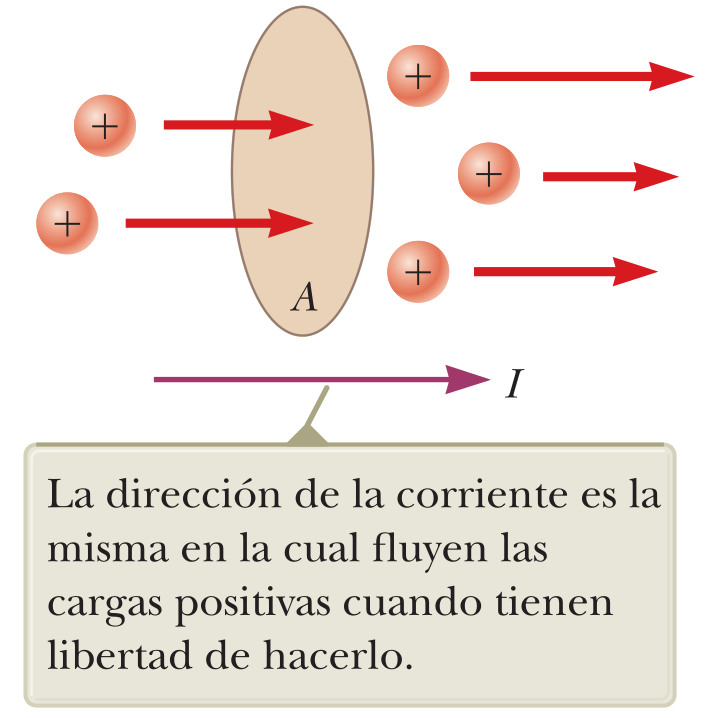
\includegraphics[width=\linewidth]{charges_flow.png}
    \caption{Cargas en movimiento a través de un área \(A\).}
    \label{fig:current}
\end{wrapfigure}

La corriente eléctrica es el flujo de carga eléctrica a través de un conductor. En un circuito eléctrico, la corriente se define como la cantidad de carga que pasa por unidad de area en un tiempo determinado. La unidad de medida de la corriente es el \hl{amperio} (\(A\)), que equivale a un culombio por segundo (\(C/s\)).

Cuando hablamos de \textbf{flujo de carga} nos referimos a la cantidad de carga que se mueve a través de una sección transversal del conductor en un tiempo determinado.

\subsubsection{Definición}

Para definir la corriente con mayor presición, suponga que las cargas tienen un movimiento perpendicular a una superficie \(A\), segun se observa en la figura \ref{fig:current}. La \textbf{corriente} se define como la tasa a la cual circula la carga a través de la superficie. Si \(\Delta Q\) es la carga que pasa a través de la superficie \(A\) en un intervalo de tiempo \(\Delta t\), la corriente promedio \(I_{prom}\) se define como:

\begin{equation}
    I_{prom} = \frac{\Delta Q}{\Delta t}
\end{equation}

Si la tasa a la que pasan las cargas varía en el tiempo, la corriente instantánea \(I\) se define como:
\[
    I = \lim_{\Delta t \to 0} \frac{\Delta Q}{\Delta t} = \frac{dQ}{dt}
\]

\begin{tcolorbox}[mydanger]
    \textbf{Cuidado:} la corriente es una magnitud \textit{escalar}. Por lo general describiremos la dirección de la corriente ya sea con palabras (por ejemplo, ``la corriente fluye por el circuito en el sentido horario'') o eligiendo una corriente como positiva si fluye en un sentido a lo largo de un conductor, y negativa si fluye en sentido contrario.
\end{tcolorbox}

\subsubsection{Movimiento de las cargas}

Para que exista un movimiento de cargas, es necesario que exista una fuerza que actúe sobre ellas. Esta fuerza es la fuerza eléctrica (ley de Coulomb: \ref{eq:ley_coulomb}) que actúa sobre las cargas libres (electrones) debido a la presencia de un campo eléctrico \(E\). Es decir, para que haya corriente eléctrica, debe existir un campo eléctrico que actúe sobre las cargas libres en el conductor. Este campo eléctrico puede ser generado por una diferencia de potencial entre dos puntos del conductor, como en el caso de una batería o una fuente de alimentación.

Cuando hay un campo eléctrico en un conductor, las cargas libres se aceleran y adquieren una velocidad. En palabras simples, podemos asociar la corriente eléctrica con el movimiento de cargas libres en un conductor.

En un conductor, los electrones libres se mueven en direcciones aleatorias debido a la temperatura del material. Sin embargo, cuando se aplica un campo eléctrico, estos electrones adquieren una velocidad de arrastre o \textbf{velocidad de deriva} \(v_d\) en la dirección del campo eléctrico. La velocidad de deriva es la velocidad promedio de las cargas (electrones en el caso de un conductor).

\begin{figure}[ht]
    \centering
    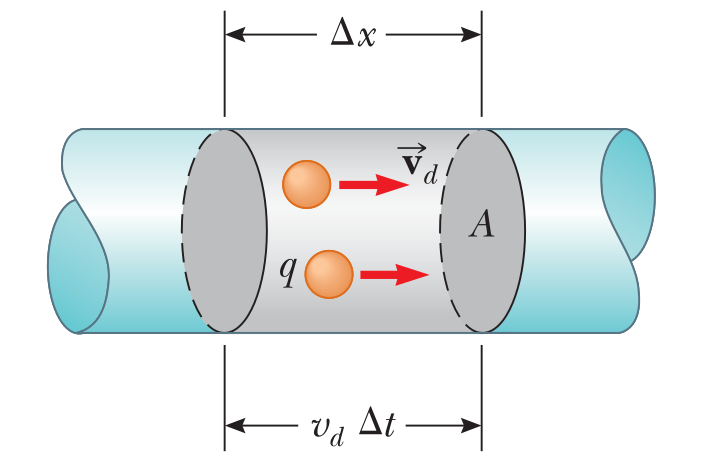
\includegraphics[width=0.5\textwidth]{v_d.png}
    \caption{Movimiento de cargas en un conductor.}
    \label{fig:movimiento_de_cargas_en_un_conductor}
\end{figure}

Recordando que \(\Delta Q\) es la cantidad de carga que pasa a través de la sección transversal \(A\), si tomamos un pedazo de conductor de longitud \(\Delta x\) como se muestra en la figura \ref{fig:movimiento_de_cargas_en_un_conductor}, podemos expresar el volúmen de este segmento de conductor como \(A \, \Delta x\). Si \(n\) es la densidad de carga (número de cargas por unidad de volumen), el número de cargas en el segmento es \(n A \Delta x\). Entonces la carga total de esta sección es:
\[
    \Delta Q = (n \, A \, \Delta x) \, q
\]
donde \(q\) es la carga de cada portador. Si tomamos un intervalo de tiempo \(\Delta t\) y consideramos que la velocidad promedio de las cargas es \(v_d\), el desplazamiento \(\Delta x\) se puede expresar como \(\Delta x = v_d \, \Delta t\). Entonces, podemos reemplazar \(\Delta x\) en la expresión de \(\Delta Q\):
\[
    \Delta Q = (n \, A \, v_d \, \Delta t) \, q
\]

Si dividimos ambos lados de la ecuación por \(\Delta t\), obtenemos la corriente promedio:
\[
    I_{prom} = \frac{\Delta Q}{\Delta t} = n \, A \, v_d \, q
\]

\begin{figure}[ht]
    \centering
    \begin{subfigure}[b]{0.4\textwidth}
        \centering
        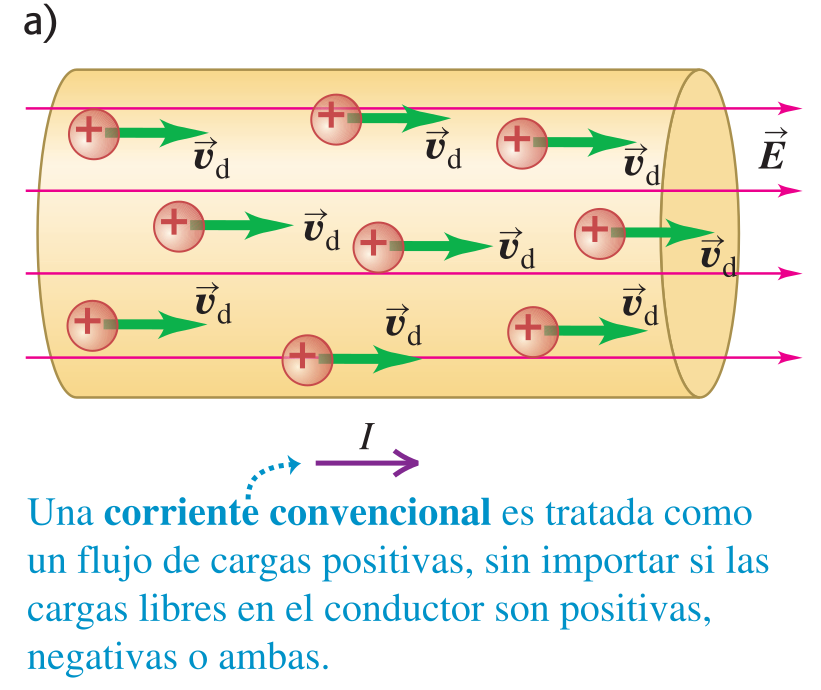
\includegraphics[width=\textwidth]{charges_movement_1.png}
        \caption{flujo de cargas positivas.}
        \label{fig:flujo_de_cargas_positivas}
    \end{subfigure}
    \hspace{10pt}
    \begin{subfigure}[b]{0.4\textwidth}
        \centering
        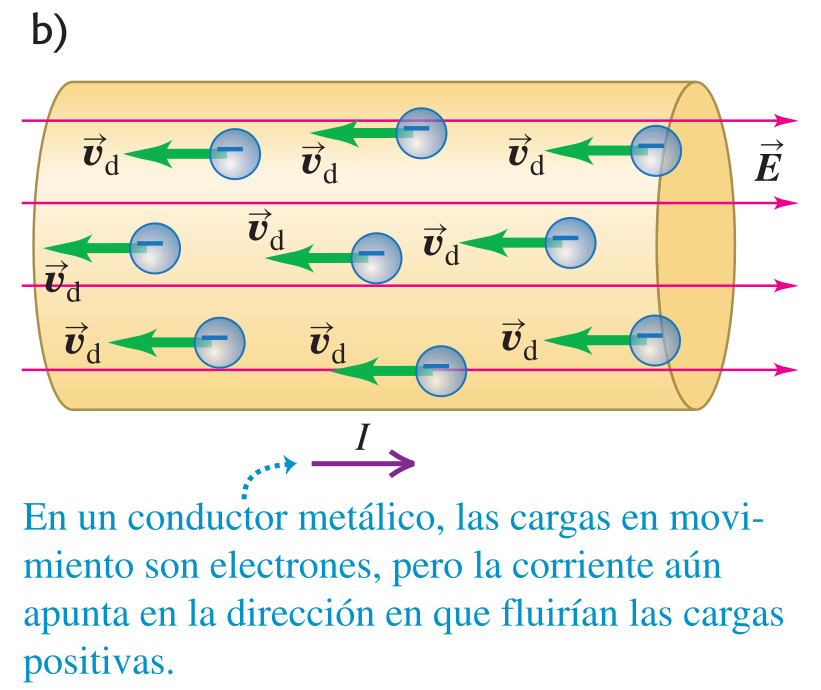
\includegraphics[width=\textwidth]{charges_movement_2.png}
        \caption{flujo de cargas negativas.}
        \label{fig:flujo_de_cargas_negativas}
    \end{subfigure}
    \caption{Flujo de cargas en un conductor.}
    \label{fig:flujo_de_cargas}
\end{figure}

La figura \ref{fig:flujo_de_cargas} presenta segmentos de material conductor. En la figura \ref{fig:flujo_de_cargas_positivas}, las cargas en movimiento son positivas, la fuerza eléctrica ocurre en la misma dirección que \(E\), y la velocidad de deriva \(v_d\) es de izquierda a derecha. En la figura \ref{fig:flujo_de_cargas_negativas} las cargas son negativas, la fuerza eléctrica es opuesta a \(E\), y la velocidad de deriva \(v_d\) es de derecha a izquierda. Definimos que la corriente, denotada por \(I\), va en la dirección en la que hay un flujo de carga positiva. Por ello, las corrientes se describen como si consistieran por completo en un flujo de cargas positivas, aun en los casos en que se sabe que la corriente real se debe a electrones. Así, en las figuras \ref{fig:flujo_de_cargas_positivas} y \ref{fig:flujo_de_cargas_negativas} la corriente es hacia la derecha. Esta convención sobre la dirección del flujo de la corriente se llama \textbf{corriente convencional}. Aunque la dirección de la corriente convencional no es necesariamente la misma en que se desplazan en realidad las partículas con carga, veremos que el signo de las cargas en movimiento tiene poca importancia en el análisis de los circuitos eléctricos.

\subsubsection{Densidad de corriente}

La densidad de corriente \(\vec{J}\) se define como la corriente por unidad de área transversal:
\[
\vec{J} = \frac{I}{A} \vec{u}
\]
donde \( I \) es la corriente, \( A \) es el área y \( \vec{u} \) es un vector unitario en la dirección del flujo de corriente.

Dado que la corriente \(I\) se puede expresar como \(n \, A\, v_d\, q\), la densidad de corriente se puede expresar como:
\[
\vec{J} = n q \vec{v}_d
\]

Es importante notar que la densidad de corriente es un vector, pero la corriente \(I\) no lo es. La diferencia está en que la densidad de corriente \(\vec{J}\) describe como fluyen las cargas en cierto punto, mientras que la corriente \(I\) describe la forma en la que fluyen las cargas a través de un objeto extendido. 

\subsection{Ley de Ohm}

\subsubsection{Resistividad}

La \textbf{resistividad} \(\rho\) de un material se define como la razón de las magnitudes del campo eléctrico y la densidad de corriete:
\begin{equation}
    \rho = \frac{E}{J} \quad [\Omega \cdot m]
\end{equation}

El recíproco de la resistividad es la conductividad \(\sigma\). Sus unidades son \((\Omega \cdot m)^{-1}\).
\begin{tcolorbox}[myconclusion]
\textbf{Importante:} Tanto la resistividad como la conductividad dependen del material y de factores como la temperatura.
\end{tcolorbox}

Tan pronto como se mantiene una diferencia de potencial a través del conductor se establece una densidad de corriente y un campo eléctrico. En algunos materiales, la densidad de corriente es proporcional al campo eléctrico:
\begin{equation}
\vec{J} = \sigma \vec{E} \qquad \leftrightarrow \qquad \vec{E} = \rho \vec{J}
\label{eq:forma_local_de_la_ley_de_ohm}
\end{equation}
donde la constante de proporcionalidad \(\sigma\) es la \textbf{conductividad} del conductor (\(1/\rho\)).

La relación de la ecuación \ref{eq:forma_local_de_la_ley_de_ohm} describe cómo un campo eléctrico induce una corriente en un medio conductor. Los materiales que obedecen dicha relación siguen la \textbf{ley de Ohm}.

\subsubsection{Formulando la ley de Ohm}

En estado estacionario, el campo eléctrico dentro de un conductor es constante en el tiempo. De la electrostática sabemos que:

\[
\Delta V = E \, d
\]

En un conductor rectilíneo y uniforme de longitud \( L \), la diferencia de potencial \( \Delta V \) entre sus extremos genera un campo uniforme, y despejando el campo en la ecuación anterior resulta:
\[
E = \frac{\Delta V}{L}
\]
Si el conductor tiene un área de sección transversal constante \( A \), y utilizando \( \vec{J} = \sigma \vec{E} \), la corriente total se deduce integrando la densidad de corriente sobre el área:
\[
I = \int_A \vec{J} \cdot d\vec{A} = J A = \sigma E A = \sigma \frac{\Delta V}{L} A
\]
De aquí se deduce la ley de Ohm macroscópica:
\begin{equation}
    \boxed{I = \frac{\sigma A}{L} \Delta V}
    \label{eq:ley_de_ohm}    
\end{equation}

\subsubsection{Resistencia}

La resistencia eléctrica se define como:
\[
R = \frac{\Delta V}{I} = \frac{L}{\sigma A}
\]

La inversa de la conductividad es la resistividad \( \rho \), por lo tanto:

\begin{equation}
    \boxed{R = \rho \frac{L}{A}}
    \label{eq:resistencia}
\end{equation}

\subsection{Aplicación de la ley de Ohm a circuitos}

\subsubsection{Circuitos en Serie}

Antes de comenzar es importante tener en cuenta que en un circuito en serie la corriente \( I \) es la misma en todos los elementos debido a que no hay bifurcaciones. Esto es debido a la conservación de la carga eléctrica y a la naturaleza de la conexión en serie.

Para entenderlo desde un enfoque físico, cuando varios elementos (resistencias, capacitores, etc.) están conectados en serie, sólo hay un camino posible para que circule la corriente eléctrica. Esto significa que las cargas eléctricas (generalmente electrones en un conductor metálico) no tienen bifurcaciones o alternativas en su trayecto: todas las cargas que pasan por un punto del circuito deben pasar por todos los demás puntos sucesivos en la misma rama.

Aplicando la ley de conservación de la carga (una consecuencia directa de la ley de continuidad en electromagnetismo), se deduce que no puede haber acumulación de carga en ningún punto del conductor en estado estacionario. Por tanto, el flujo de carga (es decir, la corriente) debe ser constante en todos los elementos conectados en serie. Si no fuera así, habría acumulación o desaparición de carga en algún nodo, lo cual no ocurre en un circuito cerrado en régimen permanente.

Es como el flujo de agua en una fuente; el agua brota de la parte superior de la fuente al mismo ritmo con el que llega a la parte inferior, sin importar las dimesiones de la fuetne. ¡El agua no ``se gasta'' a lo largo del trayecto!

En base a esta premisa, para cada resistencia, se cumple:

\[
V_i = I R_i
\]

La ley de Kirchhoff de tensiones establece que la suma de las caídas de potencial en una malla cerrada es igual a la fuente de tensión aplicada:

\[
V = V_1 + V_2 + \cdots + V_n = IR_1 + IR_2 + \cdots + IR_n
\]

Factorizando la corriente \( I \):

\[
V = I (R_1 + R_2 + \cdots + R_n)
\]

Definiendo la resistencia equivalente \( R_{\text{eq}} \) del sistema:

\[
\boxed{R_{\text{eq}} = R_1 + R_2 + \cdots + R_n}
\]

\paragraph{Ejemplo sencillo:}

Tres resistencias: \( R_1 = 2 \, \Omega \), \( R_2 = 3 \, \Omega \), \( R_3 = 5 \, \Omega \)

\[
R_{\text{eq}} = 2 + 3 + 5 = 10 \, \Omega
\]

Si se aplica una diferencia de potencial de \( V = 20 \, \text{V} \), entonces:

\[
I = \frac{V}{R_{\text{eq}}} = \frac{20}{10} = 2 \, \text{A}
\]

\subsubsection{Circuitos en Paralelo}

Al igual que en la sección anterior, vamos a partir con algunos supuestos físicos:
\begin{itemize}
    \item Las resistencias \( R_1, R_2, ..., R_n \) están conectadas en paralelo tienen sus terminales conectadas a los mismos dos nodos.
    \item La diferencia de potencial \( V \) es la misma en cada una.
    \item La corriente total se divide entre las ramas: \( I = I_1 + I_2 + \cdots + I_n \)
\end{itemize}

Entonces, aplicando la ley de Ohm y de la ley de Kirchhoff de corrientes

En cada resistencia, se cumple:

\[
I_i = \frac{V}{R_i}
\]

La corriente total será:

\[
I = \frac{V}{R_1} + \frac{V}{R_2} + \cdots + \frac{V}{R_n}
\]

Factorizando \( V \):

\[
I = V \left( \frac{1}{R_1} + \frac{1}{R_2} + \cdots + \frac{1}{R_n} \right)
\]

Definimos \( R_{\text{eq}} \) como la resistencia que satisface \( I = \frac{V}{R_{\text{eq}}} \). Entonces:

\[
\frac{V}{R_{\text{eq}}} = V \left( \sum_{i=1}^{n} \frac{1}{R_i} \right)
\Rightarrow \boxed{\frac{1}{R_{\text{eq}}} = \frac{1}{R_1} + \frac{1}{R_2} + \cdots + \frac{1}{R_n}}
\]

\paragraph{Ejemplo sencillo:}

Tres resistencias: \( R_1 = 4 \, \Omega \), \( R_2 = 6 \, \Omega \), \( R_3 = 12 \, \Omega \)

\[
\frac{1}{R_{\text{eq}}} = \frac{1}{4} + \frac{1}{6} + \frac{1}{12} = \frac{3 + 2 + 1}{12} = \frac{6}{12} = \frac{1}{2}
\Rightarrow R_{\text{eq}} = 2 \, \Omega
\]

\subsection{Energía y Potencia eléctrica}

Ahora abordaremos las expresiones teóricas de energía y potencia eléctrica en un circuito de corriente continua, partiendo de principios fundamentales. Estas magnitudes están directamente relacionadas con el trabajo que realiza el campo eléctrico sobre las cargas en movimiento. 

\subsubsection{Trabajo eléctrico}

Recordando lo que vimos en la unidad de electrostática, cuando una carga eléctrica \( q \) se desplaza entre dos puntos con diferencia de potencial \( \Delta V \), el trabajo realizado por el campo eléctrico es:

\[
W = q \Delta V
\]

Este trabajo es la energía transferida al sistema. Si en lugar de una sola carga \(q\) consideramos una corriente continua \( I \), que representa el flujo de carga por unidad de tiempo podríamos calcular el trabajo realizado por la corriente de cargas, entonces partir de la definición de corriente operamos para obtener una expresión para \(q\):

\begin{align*}
    I &= \frac{\Delta q}{\Delta t} \\
    I \Delta t &= \Delta q \\
    \Delta q &= I \Delta t
\end{align*}

Entonces, el trabajo realizado en ese intervalo de tiempo es:

\begin{equation}
    W = I \Delta V \, \Delta t
    \label{eq:trabajo_electrico}    
\end{equation}

\subsubsection{Potencia eléctrica}

La potencia es el trabajo realizado en un intervalo de tiempo, entonces la tasa de transferencia de energía (o trabajo realizado) por unidad de tiempo es:

\[
P = \frac{dW}{dt}
\]

Sustituyendo la expresión anterior para \( W \), obtenemos:

\begin{align}
    P &= \frac{d}{dt}(I \Delta V \, \Delta t) = I \Delta V \notag \\
    P &= IV
\end{align}

Esta expresión nos indica la potencia disipada (si \( V \) e \( I \) tienen el mismo signo) o suministrada (si tienen signos opuestos) en un componente del circuito.

Aplicando la ley de Ohm (\( V = IR \)) a la ecuación de potencia podemos encontrar la potencia disipada en una resistencia:

\[
P = VI = (IR)I = \boxed{P = I^2 R}
\]

Alternativamente, despejando la corriente de la ley de Ohm:

\[
I = \frac{V}{R} \Rightarrow P = V \left( \frac{V}{R} \right) = \boxed{P = \frac{V^2}{R}}
\]

Estas tres expresiones son equivalentes:

\begin{equation}
    \boxed{P = VI = I^2 R = \frac{V^2}{R}}
    \label{eq:potencia_electrica}
\end{equation}

y se usan dependiendo de qué variables sean conocidas en un circuito dado.


\subsubsection{Energía disipada en el tiempo}

Integrando la potencia en el tiempo se obtiene la energía total disipada o entregada:

\[
W = \int_{t_0}^{t_1} P \, dt = \int_{t_0}^{t_1} VI \, dt
\]

Si el circuito opera bajo condiciones constantes (circuito de corriente continua pura), entonces:

\[
W = V I \Delta t
\]

Si la resistencia es la única componente significativa, entonces:

\[
W = I^2 R \Delta t = \frac{V^2}{R} \Delta t
\]


\paragraph{Ejemplo sencillo}

Un resistor de \( R = 10 \, \Omega \) conectado a una batería de \( V = 12 \, \text{V} \), durante \( \Delta t = 30 \, \text{s} \).
\begin{itemize}
    \item Corriente: \( I = \frac{V}{R} = \frac{12}{10} = 1.2 \, \text{A} \)
    \item Potencia disipada: \( P = I^2 R = (1.2)^2 \cdot 10 = 14.4 \, \text{W} \)
    \item Energía disipada: \( W = P \Delta t = 14.4 \cdot 30 = 432 \, \text{J} \)
\end{itemize}

\subsection{Resumen}
\begin{tcolorbox}[title=Corriente Eléctrica]
  La corriente eléctrica es la tasa a la cual circula la carga a traves de una superficie.
  \[
    I_{prom} = \frac{\Delta Q}{\Delta t}
  \]
  que puede relacionarse con el movimiento de las cargas:
  \[
    I_{prom} = n q v_d A
  \]

  De esta ecuación se puede obtener la velocidad a la cual circulan los portadores de carga. La velocidad de deriva o arrastre es:
  \[
    v_d = \frac{I}{nqA}
  \]
  donde:
  \begin{itemize}
    \item \(I\) es la corriente que circula por el material
    \item \(q\) es la carga de los portadores (\(e=1.6\times10^{-19}\) en el caso de los electrones)
    \item \(A\) es el área transversal del material
    \item \(n\) es la densidad de portadores (el número de portadores) del el material por unidad de volumen.
  \end{itemize}

  Para obtener \(n\) para un material dado podemos usar la siguiente aproximación:
  \[
    n=\frac{\delta}{m_{molar}} N_A
  \]
  donde:
  \begin{itemize}
    \item \(\delta\) es la densidad del material
    \item \(m_{molar}\) es la masa molar del material
    \item \(N_A = 6.022 \times 10^{23} \, \mathrm{mol}^{-1}\) es el número de Avogadro.
  \end{itemize}
\end{tcolorbox}

\begin{tcolorbox}[title=Ley de Ohm]
  La ley de Ohm establece una relación de proporcionalidad entre la corriente, el potencial y la resistencia:
  \[
    V = IR
  \]
  \begin{itemize}
    \item La densidad de corriente es: \(\vec{J} = \sigma \vec{E}\)
    \item Ley de Ohm macroscópica: \(I = \frac{\sigma A}{L} \Delta V\)
    \item Definición de resistencia: \(R = \frac{\Delta V}{I} = \rho \frac{L}{A}\)
    \item Relación entre corriente y densidad de corriente: \(I = \int_A \vec{J} \cdot d\vec{A}\)
  \end{itemize}
  Estas ecuaciones permiten modelar y analizar cualquier sistema de corriente continua en conductores ohmicos.
\end{tcolorbox}


\begin{tcolorbox}[title=Circuitos]
  \subparagraph{Serie:}
  \begin{itemize}
    \item Corriente común: \( I = \text{constante} \)
    \item Tensión total: \( V = V_1 + V_2 + \cdots + V_n \)
    \item Resistencia equivalente: \(R_{\text{eq}} = \sum_{i=1}^{n} R_i\)
  \end{itemize}
  
  \subparagraph{Paralelo:}
  \begin{itemize}
    \item Tensión común: \( V = \text{constante} \)
    \item Corriente total: \( I = I_1 + I_2 + \cdots + I_n \)
    \item Resistencia equivalente: \(\frac{1}{R_{\text{eq}}} = \sum_{i=1}^{n} \frac{1}{R_i}\)
  \end{itemize}
\end{tcolorbox}


\begin{tcolorbox}[title=Trabajo y Potencia eléctrica]
  \subparagraph{Potencia general:}  
  
  \[
    P = V I
  \]
  
  \subparagraph{Potencia disipada en resistencias:}  
  \[
    P = I^2 R = \frac{V^2}{R}
  \]
  
  \subparagraph{Energía disipada o entregada en el tiempo \( \Delta t \):}
  \[
    W = P \Delta t = V I \Delta t = I^2 R \Delta t = \frac{V^2}{R} \Delta t
  \]
\end{tcolorbox}
